% Change to use the correct class file for your paper.
\documentclass{sig-alternate-10pt}

%\pagenumbering{arabic}

\usepackage{amsfonts}     % Adds math fonts, commands such as \begin{align}
\usepackage{array}        % Tables for use in math mode
\usepackage{booktabs}     % Elegant table-formatting library
\usepackage{bold-extra}   % Provides bf+sc (only in textbf+textsc env.)
\usepackage{bytefield}    % Formatting and layout of packets / bytefields
\usepackage[skip=5pt]{caption}
\usepackage{color}        % Allow the use and definition of colors
\usepackage{colortbl}     % Color table cells
\usepackage{comment}      % Provides \begin,\end{comment} for large blocks
%\usepackage{cprotect}     % Allows verbatim, other formatting in macro args
\usepackage{endnotes}     % Footnotes pushed to the end of a document
\usepackage{gensymb}      % Adds useful symbols w/out math mode, e.g. \degree
\usepackage{graphicx}     % For importing graphics
\usepackage{hyperref}     % Creates hyperlinks from ref/cite 
\hypersetup{pdfstartview=FitH}
\usepackage{listings}     % in-line source code (poorly, consider minted)
\usepackage{mathtools}    % amsmath extension, adds more math formatting
\usepackage{multirow}     % Multiple row spacing in tables
\usepackage{nth}          % Typeset 33rd correctly as \nth{33}
%\usepackage[section]{placeins} % Don't let figs escape their sections
\usepackage{rotating}     % Rotates any object, note sideways != sidewaysfigure
%\usepackage[all=normal]{savetrees} % For when space is tight, read manual and
                          % selectively enable things. CAN BREAK CONF STYLES!!
\usepackage{soul}         % Provides \hl{} for highlighting
%\usepackage{subfig}
%\usepackage{subfigure}    % Complicated figure creation
\usepackage{subcaption}   % Replaces both subfig and subfigure
\usepackage[nofancy]{svninfo} % svn information in docs (req. svn:keywords)
\usepackage{tabularx}     % Complicated table creation
\usepackage{threeparttable} % Add footnotes to a table
\usepackage{units}        % For nice fractions, \nicefrac{1}{2} --> 1/2
\usepackage{url}          % Pretty printing of hyperlinks
\usepackage{xspace}       % Intelligently add spaces after commands

%%%%%
% used in QxDM section
\usepackage{epstopdf}
\epstopdfsetup{update}
\usepackage{algorithmic}
\usepackage{algorithm}
\usepackage{array}
\usepackage{tabularx}
%%%%%

\usepackage{epsfig,xspace,multirow,capt-of}
\usepackage{hyperref}
\usepackage{graphicx,amssymb,amsmath,endnotes}
\usepackage{times}
\usepackage{ulem}
\usepackage{rotating}
\usepackage{wasysym, pifont}

\DeclareCaptionType{copyrightbox}

\newlength\SUBSIZE

\renewcommand{\arraystretch}{1.2} % Space out rows in tables

%\setlength\paperheight {11in}
%\setlength\paperwidth {8.5in}

\hyphenpenalty=800
\tolerance=400

% italics for bibliography
\normalem


%%%%%
% new command
\newcommand{\MR}[1]{\multirow{2}{*}{#1}}

\newcommand{\mysection}[1]{\vspace{-.07in}\section{#1}\vspace{-.02in}}
\newcommand{\mysubsection}[1]{\vspace{-.05in}\subsection{#1}\vspace{-.02in}}
\newcommand{\mysubsubsection}[1]{\vspace{-.05in}\subsubsection{#1}\vspace{-.02in}}


\newcommand{\hd}[1]{\small{\textbf{\texttt{#1}}}\normalsize}
\newcommand{\hds}[1]{\small{\textbf{\texttt{#1}}}}
\newcommand{\hdf}[1]{\small{\textbf{\texttt{#1}}}\footnotesize}

\newcommand{\ISP}{$\sf\small{ISP}$}
\newcommand{\ISPP}{$\sf\small{ISP}$ }
\newcommand{\UMICH}{$\sf\small{UMICH}$}
\newcommand{\UMICHH}{$\sf\small{UMICH}$ }

\newcommand{\YY}{\CIRCLE}
\newcommand{\NN}{\Circle}
\newcommand{\YN}{\RIGHTcircle}
\newcommand{\XX}{\ding{53}}

\newcommand{\Ignore}[1]{{\small }}
\definecolor{gray}{rgb}{0.5,0.5,0.5}
\newcommand{\etc}{\emph{etc.}\xspace}
\newcommand{\ie}{\emph{i.e.,}\xspace}
\newcommand{\eg}{\emph{e.g.,}\xspace}
\newcommand{\etal}{\emph{et al.}\xspace}
\newcommand{\wrt}{\emph{w.r.t.}\xspace}
\newcommand{\aka}{\emph{a.k.a.}\xspace}
\newcommand{\AlgBox}[1]{{\framebox[1.2\width]{\textbf{#1}}}}
\newcommand{\mycomment}[1]{{\color{red}[\textsf{#1}]}}

\renewcommand{\paragraph}[1]{\smallskip\noindent{\bf{#1.}}}
\newcommand{\paragrapha}[1]{\smallskip\noindent{\bf{#1}}}
%\renewcommand{\algorithmiccomment}[1]{//#1}

\makeatletter
  \newcommand\figcaption{\def\@captype{figure}\caption}
  \newcommand\tabcaption{\def\@captype{table}\caption}
\makeatother

\newcommand{\vsp}{\vspace{+0.15in}}

\newcommand{\nsection}[1]{\vspace{-1em}\section{#1}\vspace{-0.7em}}
\newcommand{\nsubsection}[1]{\vspace{-0.85em}\subsection{#1}\vspace{-0.55em}}
\newcommand{\nsubsubsection}[1]{\vspace{-0.4em}\subsubsection{#1}\vspace{-0.3em}}
\newcommand{\ncaption}[1]{
 	\vspace{-1.2em}
	\caption{#1}
 	\vspace{-1.5em}
}
%%%%%


\begin{document}

\title{TransLayer: A Root Cause Identification Tool for Analyzing Cellular Abnormal Behaviors}

% AUTHOR STYLE 1
%\author{
% \alignauthor{Haokun Luo}\\
% \affaddr{University of Michigan}\\
% \email{\{haokun\}@umich.edu}
%}

% AUTHOR STYLE 2
\author{
Haokun Luo$^\dagger$, Z.~Morley Mao$^\dagger$, Kranthi Sontineni$^\natural$, Jie Hui$^\natural$, 
 Kevin Lau$^\natural$\\
$^\dagger$University of Michigan, $^\natural$T-Mobile USA Inc.
} % end author

\conferenceinfo{T-mobile User Intelligent Project} {Sep 03 -- Nov 30, 2013, Ann Arbor, Michigan, USA.}
\CopyrightYear{2013}

\maketitle

\begin{abstract}
% ABSTRACT

Slow network experience on smartphone could hurt user experience and downgrade application reputation. When users are urgent about specific information, the carried information size is small but the latency of the mobile network service is very sensitive. The discontinuous burst of short data transmission is the most common traffic pattern in the cellular network. But significant latency appears at the beginning part of the data transmission. In order to identify the root cause, I use diagnostic cross layer monitoring tool, QxDM (Qualcomm eXtensible Diagnostic Monitor), and found that inactive response to packet loss in the RLC (Radio Link Resource) leads to unnecessary timeout in the transport layer. I propose a RLC \textit{Fast Re-Tx (Retransmission)} mechanism to avoid sluggish reaction to packet loss, and further reduce the latency during the initial network connection. Based on our simulation results, the \textit{Fast Re-Tx} mechanism could reduce the latency by up to \textit{35.69\%} over initial network connection.


\end{abstract}


\terms{Mobile, Measurement, QoE, Tool}
\keywords{LTE, WCDMA, RRC, RLC, Cross-layer Analysis, Root Cause Analysis, Real-time User Feedback}

%\newpage

% page limit          % 14.0 pg
% abstract            %  0.5 pg
%\vfill\eject
\section{Introduction}
%\renewcommand{\labelitemii}{$\star$}
Cellular network technologies, such as 3G \textit{Universal Mobile Telecommunications System} (UMTS) and 4G \textit{Long Term Evolution} (LTE), require that devices transition between various RRC states based on the network traffic patterns of individual mobile clients.  These states have different performance and energy consumption tradeoffs, as well as different state transition delays.  Using high-power RRC states only when necessary allows users to experience good network performance on resource-constrained mobile devices. Although the RRC states are defined by \textit{3rd Generation Partnership Project} (3GPP)~\cite{spec-3G-RRC, spec-LTE-RRC}, many aspects of the RRC state machine, such as timers for transitioning between states, are implementation or configuration-specific, differing by device model, network operator and location.  The real-world deployment of RRC state machines and the impact on performance are not well-understood. 

A better understanding of RRC state behavior would be beneficial for many parties.  Cellular network operators would be interested in determining how devices on their networks perform and how performance can be improved.  Device manufacturers would be interested in detecting device-dependent effects --- device implementation details and features such as Fast Dormancy~\cite{fast_dormancy} can mean different devices perform differently. Developers of major applications might be interested in understanding how network behavior can impact application performance, as work has been done to show that application behavior can decrease RRC-related performance issues~\cite{aro}.  Finally, researchers studying protocol optimization would find a better understanding of RRC state behavior valuable. 

In this paper, we examine how RRC states are implemented, behave and perform in real-world implementations. We present a new approach to inferring RRC state transitions that addresses limitations in previous work which prevent inference from being done in non-ideal network conditions or by non-expert users. In particular, we focus on detecting performance anomalies caused by RLC-layer \textit{transient states}, which can have a significant performance impact. We perform a study of RRC state implementations and performance on 16 network operators from 9 countries,  and use RLC layer analysis to understand the root causes of behavior and performance trends discovered. We present three main categories of contributions: %. First, we present several methodological contributions which allow us to perform measurements that lead to a deeper understanding of RRC behavior. Second, we present our findings on previously unknown performance problems and phenomena. Third, we suggest some potential performance optimizations. 

%\begin{enumerate}[noitemsep,topsep=0pt,parsep=0pt,partopsep=0pt]
%[noitemsep,topsep=0pt,parsep=0pt,partopsep=0pt]
%\item
\noindent\labelitemi\indent \textbf{Methodological contributions.} We have created two types of tools. First, we designed a novel generic RRC state model inference method that is robust to poor network conditions and interfering background traffic on the mobile device. It is implemented in an Android application and is designed to be usable out of the box by non expert users.  We focus primarily on inferring the demotion timers of RRC states as well as the performance associated with each state. We hope to release this tool as open-source software. Second, we determined methods to effectively make use of RLC-layer traces from \textit{Qualcomm eXtensible Diagnostic Monitor} (QxDM). We developed a novel cross-layer mapping mechanism that correlates transport layer packets with data layer link \textit{protocol data units} (PDUs, the smallest data transmission unit in RLC). It can successfully map 99.8\% of transport-layer packets to PDUs. This allows the root causes of TCP and UDP performance and packet loss issues to be accurately identified at the RLC layer.

%\item
\noindent\labelitemi\indent  \textbf{New Findings on the Impact of RRC State on Performance.} We analyze the RRC state implementation and associated performance characteristics for a number of network operators, showing that our methods are useful in understanding RRC states in the real world. We present several new findings that show there are significant undetected performance problems in networks today. At the RLC layer, we show that there are frequent RLC-layer retransmission delays surrounding \textit{transient states}, especially during state transitions to and from FACH. 

%\item 
\noindent\labelitemi\indent \textbf{Proposed Solution to Performance Problems Found.} We propose an improvement to how RLC currently behaves based on our improved understanding of RLC-level behavior. To reduce potentially unnecessary retransmissions that occur during poorly-performing FACH-related transient states, we propose an RLC \emph{Fast Re-Tx} mechanism that actively responds to the RLC PDU loss signals. By simulating this fast retransmission mechanism using real QxDM traces that provide visibility of RLC traffic behavior, we find that our proposed mechanism could reduce RLC latency by up to 35.69\% when these poorly-performing FACH states occur. In other states, the latency is still reduced by 2.66\% on average.

% The possible latency overhead occurs when we fail to speculate the RLC retransmission, but the overall latency could still be reduced by 2.66\%.
%\end{enumerate}


%%	\begin{itemize}
%		\item
%			\textbf{Methodology:} Based on state of art RRC state inference method, we designed a generic RRC state model generation mechanism to effectively reduce the effect of unstable wireless channel, and produce finer RRC state machine using classic statistical method. In additional, we develop the first cross layer mapping mechanism in the empirical study to correlate the transport layer packets with the data layer link PDUs, so that we could accurately identify the TCP/UDP performance issue inside the RLC layer. We could map 99.8\% of the transport layer packets to the corresponding RLC layer PDUs.
%		\item
%			\textbf{Observation:} We observe the abnormal large FACH state latency issue through our RRC inference measurement. After a world wide scale deployment of RRC state model generation measurement, we are able to discover the device dependent and network specific abnormal FACH state behaviors. We also observe the frequent RLC layer retransmission and retransmission delay over initial FACH state and FACH promotion transition, which contributes a lot to the transport layer latency.
%		\item	
%			\textbf{Implications:} Due the abnormal initial FACH state and FACH latency behavior, the application could batch the data transmission to reduce the possible number of transmission over FACH. To address the RLC retransmission delay issue, we propose a RLC \emph{Fast Re-Tx} mechanism to active response to the RLC PDU loss signals. By simulate the fast retransmission mechanism in the real trace QxDM, we apply cost-benefit analysis and found that \emph{Fast Re-Tx} could reduce RLC latency up to 35.69\% over FACH states.
%	\end{itemize}
         % 1.5 pg
\section{Background}
\label{sec:background}

\begin{figure}[t!]
\centering
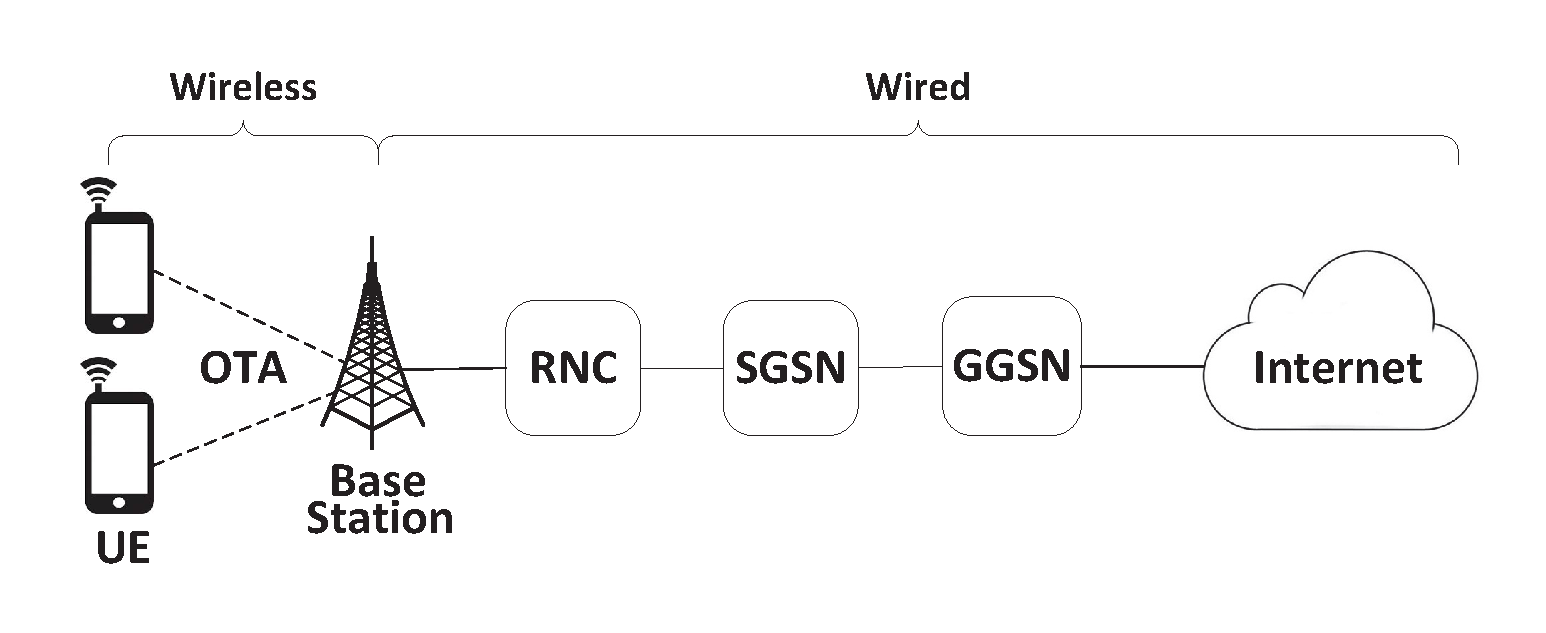
\includegraphics[width=0.5\textwidth]{figs/cellular_network_topology.eps}
\caption{The general cellular network architecture}
\label{fig:cell.topology}
\end{figure}

As illustrated in Figure~\ref{fig:cell.topology}, in both 3G UMTS~\cite{3gpp.3G} and 4G LTE networks~\cite{3gpp.LTE}, data is transmitted from \textit{user equipment} (UE), i.e. mobile devices,  to the base station (Node B in UMTS, eNB in LTE), then to the \textit{Serving GPRS support node} (SGSN) and \textit{Gateway GPRS support node} (GGSN), and ultimately to the server~\cite{umts_book}. The link between the UE and the base station is known as the \textit{over-the-air} (OTA) link, and it is the only wireless link in the network topology. The rest of the links from the base station to the internet are all wired.

\subsection{Radio Resource Control} 
\label{subsec:background.rrc}
\begin{figure}[t!]
\centering
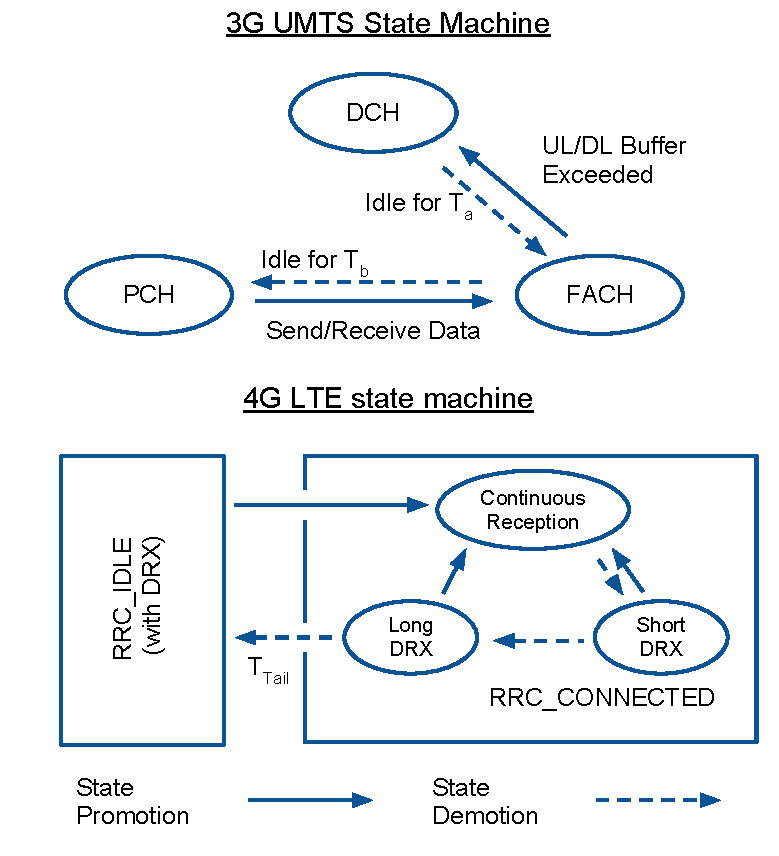
\includegraphics[width=0.5\textwidth]{figs/RRC_State_Diagram.pdf}
\caption{Possible 3G and 4G State Machines as Specified by 3GPP.} 
\label{fig:statemachine}
\end{figure}

Mobile cellular networks use the RRC protocol as the control plane signaling for Layer 3 to allocate resources to mobile devices.  Handsets transition between different RRC states, which vary in power consumption and bandwidth, and an individual RRC state machine is maintained for each handset.  Transitions between different states occur due to traffic patterns between the device and base station. In general, more traffic will cause a higher-power and higher-bandwidth state to be entered.  The RRC protocol for these network types has been defined by 3GPP~\cite{spec-3G-RRC, spec-LTE-RRC}.

For 3G UMTS~\cite{spec-3G-RRC}, there are three main states:  DCH, which is high-power and high-bandwidth, FACH, which is low power and low bandwidth, and PCH, where no transmission is possible. If a higher-bandwidth state is needed, there is a promotion delay. Some carriers may always go directly from PCH to DCH. An example RRC state machine can be seen at the top of Figure~\ref{fig:statemachine}.

For 4G~\cite{spec-LTE-RRC}, the state machine is more complicated, and is summarized in the bottom half of Figure~\ref{fig:statemachine}.  We are concerned mainly with transitions between RRC\_{}CONNECTED, a higher-power state, and RRC\_{}IDLE, a lower-power state where no data is transmitted. The other states have timers on the orders of tens or hundreds of milliseconds are are not practical to measure on end-user devices, as tools such as a power monitor are required.

\subsection{Radio Link Control}

\begin{figure}[t!]
\centering
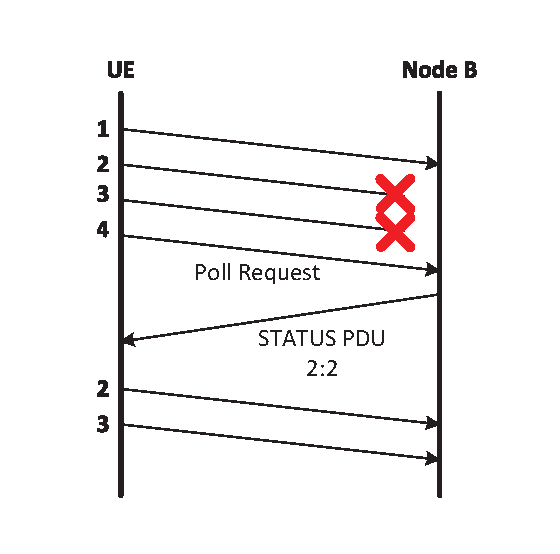
\includegraphics[width=0.5\textwidth]{figs/RLC_group_ack.eps}
\caption{RLC PDU transmission in Acknowledged Mode. When the sender sends out a polling request, the receiver will respond with a "group" of acknowledge in terms of the starting PDU sequence number and the consecutive PDU loss length.}
\label{fig:rlc.protocol}
\end{figure}

RLC protocol is a packet fragmentation protocol that used as the data plane transmission for cellular air interface~\cite{spec-3G-RLC}. There are three different modes that configured by the upper layer: TM (Transparent Mode), UM (Unacknowledged Mode), and AM (Acknowledged Mode). RLC in TM directly pass the packet from PDCP (Packet Data Convergence Protocol) layer to MAC layer, and it usually applies for voice transmission. RLC in UM sends the PDU (Packet Data Unit), which is smallest data fragmentation unit, without waiting for any response from the receiver (in this case, Node B or eNB). RLC usually transmit VoIP traffic with UM. RLC in AM deploys an ARQ (Automatic Repeat reQuest) mechanism. As show in Figure~\ref{fig:rlc.protocol}, RLC sender periodically piggybacks the polling request in the RLC header, and the receiver will respond with a RLC STATUS PDU which contains groups of not received PDU sequence numbers. We call this particular ARQ mechanism as \textit{group acknowledgement}. Since RLC transmit both TCP and UDP with AM, we will assume the rest of RLC transmission mechanism to be AM.
\label{subsec:background.rlc}
\section{Challenges}
\label{sec:challenge}

QxDM is essentially a real-time monitoring tool that connect the device with a PC (requires a USB authentication dongle). Each message or event from different layers is stored using a single log entry that has consistent format. All the analysis process is offline after we exported the filtered log information from QCAT (QualComm Analysis Tool). The first step of building cross-layer mapping of \textit{TransLayer} is to parse the trace and extract meaningful information from each log entry. Unfortunately, due to the defects of the QxDM design, incomplete RLC PDU information, loose RLC RTT estimation, and unnecessary IP packet fragmentation and duplication should be taken into consideration. For the real-time user feedback part, the most challenging component is to accurately record all the user feedback and minimize the number of incorrect signals.

\subsection{Incomplete RLC PDU Logging}
\label{subsec:partial.logging}
Due to a bad design decision, QxDM merely provides the first four bytes information in the RLC PDU for both uplink and downlink in 3G (only two bytes in LTE). Since the first two bytes PDU is constantly reserved as header, i.e. sequence number, PDU type (control PDU or data PDU), and etc, we only have two types as payload for IP packet mapping. This leads to potential unsuccessful cross-layer mapping. We provide some degree of confidence on the accuracy of mapping using uniqueness analysis ~\ref{subsec:uniqueness.analysis}, which will be covered later.

\subsection{Loose RLC RTT Estimation}
\label{subsec:loose.rlc.rtt.estimation}
In TCP, we could easily calculate the RTT (Round Trip Time) for each data packet, because each packet will be received an ACK (acknowledgement) packet except for packet loss. However, as we talked about in the \S~\ref{subsec:background.rlc}, RLC layer uses \textit{group acknowledgement} which implies not every RLC PDU could get ACK feedback from the receiver. RTT information in the lower layer is more coarse-grained compared with that of transport layer. In the future root cause analysis, we always estimate the lower layer RTT using the nearest available polling request PDU's RTT value.

\subsection{IP Fragmentation and Duplication}
\label{subsec:ip.frag.and.dup}
Although packets will be fragmented in the RLC layer because of the protocol, QxDM surprisingly breaks IP packets into units of 256 bytes without a reason. It turns out that such unnecessary fragmentation brings lots of trouble on cross-layer mapping accuracy. Another issue with IP packets is the duplication. That comes from the same IP packet payload logging twice but from different interfaces, even though you enforce the interface to be set as one of them. Therefore, pre-processing on IP log entries is quite necessary, and we evaluate the accuracy improvement to be \textit{15.24\%} in our standard \emph{Browsing Dataset} from \S~\ref{subsec:dataset}.

\subsection{Feedback Tool}
\label{subsec:challenge.feedback}
The smartphone is a very compact device that allows multiple ways for user to input their requests. However, many of the input components are well defined. Simple functionality overwrite will lead to block the normal user queries. If we create complicated input mechanism, then we might not capture all the user feedback signals. Selecting the proper interface to allow user provide feedback becomes the most challenging part of the design.
%\clearpage
%\section{Measurements}

\subsection{RRC State Inference}
The previous RRC state inference study provides a decent methodology to infer the RRC state machines~\cite{3g_rrc}. They want to infer the DCH demotion timer and FACH demotion timer in the RRC state machine. The methodology is to send a MAX (1024) bytes size packets to let the handset promote to DCH. Then wait for various amount of times (or called gap periods) to allow the handset stay in DCH, or demote to FACH, or even further demote to PCH. And send another packet with size of Max or Min (30) bytes. They measure the RTT (Round Trip Time) delay for each fixed gap period. They will infer the demotion timer by observing a larger RTT difference between two consecutive pre-defined gap periods. For example, if the RTT at gap period of 4 s is 3 times larger than that of 3.5 s, then they will conclude the FACH demotion timer is around 4 s. Since the handset will demote to FACH and promote to DCH (sending another packet) again at 4 s, the extra state transition delay contributes to the larger RTT. I repeat their experiments using UDP packets, and let the server respond an echo packets once the transmitted packet get received. In Figure~\ref{fig:rrc.infer}, I could observe an unexpected delay over FACH initial state and FACH to DCH promotion transitions, which implies the latency that mobile user could experience during the initial stage of data transmission.

% RLC Loss ratio per RRC state
\begin{figure}
\centering
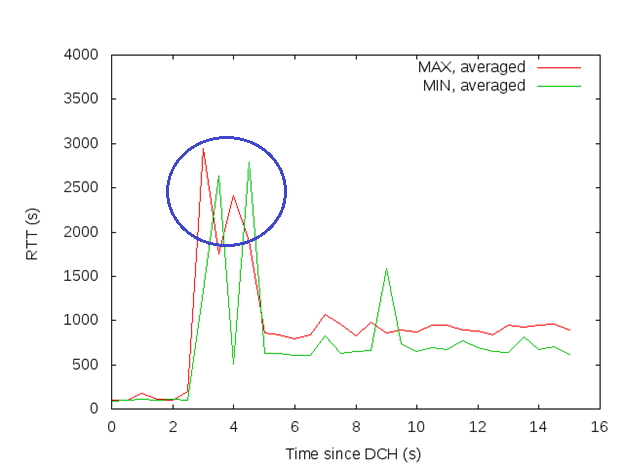
\includegraphics[width=0.45\textwidth]{figs/rrc_infer.png}
\caption{Unexpected large RTT during initial part of FACH state and FACH to DCH promotion transition}
\label{fig:rrc.infer}
\end{figure}

\subsection{Control Experiments}

% UDP/ TCP control experiment set up
The purpose of the control experiments is to verify the unexpected delays over noisy FACH state, and identify the root cause of the problem. First, we repeated our active RRC inference test for 160+ hours and dump both the client QxDM and server side tcpdump traces to perform offline analysis~\cite{tcpdump}. In order to distinguish the identities of each UDP packets, we manually injected a "sequence number" into the first four bytes of the sender's randomized payload, and the echo server sent back the received sequence number as acknowledge number in its payload. I refer the trace as \emph{UDP\_{}Trace}. Second, we designed a packet train probing using TCP packets so that we could recreate the "pseudo-state" issue~\cite{pkt.train}. Basically, we send a "train" of TCP packet size of 10 KB bytes with interleaving gap period of 3 seconds to 5 seconds incremented by 0.5 seconds with the total of 500 packets. The gap period is the DCH demotion timer period considering the variance in the lossy channel, and adjacent packet will transmit the packet starting from FACH state. Therefore, we will have more transition over the troublesome FACH state to allow us to take a closer look the root cause. Since TCP has its own ARQ (automatic repeat request) mechanism, it would be interesting to investigate the RLC retransmission's delay influence over TCP retransmission. I will refer the trace as \emph{TCP\_{}Trace}.

\label{sec:measure}

         % 3.0 pg
\section{Cross-layer Tool Design}
\label{sec:crossAnalysis}

\textit{TransLayer} is a cross-layer mapping and root cause analyzing tool based on QxDM traces. Even though it requires QxDM to gather information, we claim that such detailed lower layer information empowers us to gain a transparent view across different layers. The primary use case for \textit{TransLayer} is to identify performance issues. We talk about how to collect ground truth data transmission information in IP and RLC layer using QxDM in \S~\ref{subsec:qxdm.tool}. \S~\ref{subsec:cross-layer.mapping} talks about the core algorithm to enable cross-layer mapping between IP and RLC layer. \S~\ref{subsec:uniqueness.analysis} verifies the cross-layer mapping accuracy by showing the unique existence in the whole trace. \S~\ref{subsec:lower.layer.features} lists the major lower features that we utilize to perform root cause analysis.

\subsection{QxDM}
\label{subsec:qxdm.tool}
% Describe what the tool does
QxDM provides the the IP and lower information as input to \textit{TransLayer}. It is a real-time data collection and diagnostic logging tool for measuring mobile-based RF (Radio Frequency) performance~\cite{qxdm_flyer}. It is a Windows based monitoring application. When we perform control experiments and real application measurements, we plug in the device to the desktop or laptop with QxDM software installed. Once the experiments finishes, we filtered out the real-time monitoring information related to IP packets, RLC PDUs, and RRC states in Table~\ref{tab:QxDM.logs}, and dump the results into a log file. The 0x11EB log entry includes IP headers, IP payloads, and its customized header. Since large IP packets will be fragmented into smaller segments, the customer header could indicate the segment index of the whole IP packet. The 0x4132 and 0x4133 unveil the RLC AM configurations, i.e. the polling function timers, the retransmission limit for a single PDU, and etc. The 0x413B, and 0x418B provides RLC PDU header and first byte payload information for both data PDUs and control PDUs (or STATUS PDUs) in both uplink and downlink directions. We wrote a QxDM log parser to aggregate the filtered entries in \textit{TransLayer}, and apply cross-layer mapping to understand the correlation between different layers. We conduct all the experiments on Galaxy S3 with Android OS 4.1.1.

% Table of QxDM entries
\begin{table}[t!]
\begin{tabularx}{0.48\textwidth}{ | c | X | }
	\hline
  	\textbf{QxDM Log ID} & \textbf{Description} \\
  	\hline\hline
  	0x11EB & IP data packets \\
  	\hline
  	0x4132 & WCDMA RLC downlink acknowledge mode configuration \\
  	\hline
  	0x4133 & WCDMA RLC uplink acknowledge mode configuration \\
  	\hline
  	0x413B & WCDMA RLC uplink acknowledge mode PDU \\
  	\hline
  	0x418B & WCDMA Flexible RLC downlink acknowledge mode PDU \\
  	\hline
  	0x4125 & WCDMA RRC states \\
  	\hline
\end{tabularx}
\caption{QxDM log entries used in cross layer analysis}
\label{tab:QxDM.logs}
\end{table}

\subsection{Cross-layer Mapping}
\label{subsec:cross-layer.mapping}
% Describe the mapping algorithm I use for cross-layer analysis
QxDM tool provides fine grained lower layer RLC layer transmission information. If we could correlate the transport layer packets with the RLC layer transmitted PDUs, we will have a transparent view of the link layer behaviors, especially the RLC retransmission. As mentioned in \S~\ref{subsec:partial.logging}, one of the fundamental limitation of QxDM is the partial logging issue. For example, only the header and first byte data payload will be logged for each RLC PDU. It is also possible that a small fraction of RLC PDUs cannot be captured, which lead to a unnecessary sequence number gap. Our mapping algorithm will handle all the limitations we have mentioned.

\begin{figure}[t!]
\centering
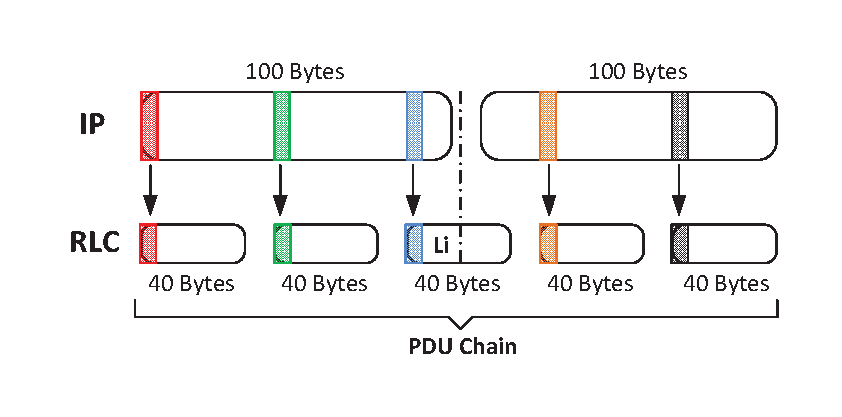
\includegraphics[width=0.5\textwidth]{figs/cross_layer_mapping.eps}
\caption{Cross-layer mapping from IP packets to RLC PDUs chains, where are a sequence of consecutive RLC PDUs. Due to the partial logging, we could only map the limited bytes for every certain length (\textit{long jump mapping}). It is possible that one PDU could concatenate the last part of the first SDU and the first part of the second SDU. Therefore, the five RLC PDU forms a unique RLC PDU chain.}
\label{fig:cross.layer.mapping}
\end{figure}

% The mapping algorithm here
The cross-layer mapping algorithm is the core technique for \textit{TransLayer}. It is essentially a map between the complete IP packets (also known as SDU) and corresponding fragmented RLC payload data bytes (known as PDU). Due to the partial logged information in QxDM, only the first data byte is captured in the log. Thus, we have to skip over the rest of the PDU, and try to match for the first data byte in the next PDU as shown in Figure~\ref{fig:cross.layer.mapping}, which we call the \textit{long jump mapping}. The problem at this point is to determine the end of IP packets while we iterate through the consecutive RLC PDUs. Since each PDU could either contain the payload data dedicated to a single SDU or belongs to two SDUs. If the reminder size of the SDU cannot fulfill the largest size of PDU, then RLC protocol will concatenate the part of the next SDU to fill the rest of space~\cite{spec-3G-RLC} using LI (Length Indicator) in the RLC PDU header. Ultimately, if the accumulative mapped index equals the size of SDU, we claim to find a mapping successfully; otherwise no mapping discovered.

% the corner case of the mapping algorithm
There is a corner case in the mapping algorithm such that the QxDM cannot capture the some of the SDUs. Similar to TCP protocol, the sequence number in RLC PDUs could uniquely distinguish between every PDUs. If there are some missed PDUs, then we cannot map the first byte data for every PDU size. In that case, we could even skip over the missed PDUs and add up multiple of PDU size to hunt for a match. Because of the limitation of the QxDM tool, the \textit{long jump mapping} mechanism cannot fully recover the corner case, especially when the missed PDUs were either the beginning or the end part of the mapped RLC list. We evaluate the improved mapping algorithm by checking the percentage of mapped IP packets in our standard \emph{Browsing Dataset} from \S~\ref{subsec:dataset}, and the average mapping ratio is \textit{99.52\%} for uplink and \textit{88.83\%} for downlink. One reason for a lower the downlink ratio is that the size of PDU is flexible in WCDMA downlink, and the average size is around 17 times greater than that of uplink in our traces. Considering the partial logging information, that actually implies fewer information is available in downlink RLC layer, which leads to a smaller successful mapping ratio.

\subsection{Uniqueness Analysis}
\label{subsec:uniqueness.analysis}
The cross-layer mapping in \S~\ref{subsec:cross-layer.mapping} only claims the existence of cross-layer, but it does not guarantee the mapped RLC PDUs exist once in the trace. We perform uniqueness analysis to prove the uniqueness of the mapped RLC PDUs in the whole trace. One important observation is that RLC SDU concatenation is fairly common as shown in Figure~\ref{fig:cross.layer.mapping}, especially during bulk transmission in transport layer. The concatenation actually introduces some degree of randomness of the partial RLC PDU payload locations. In other word, the cross-layer mapping does not always start from the very first byte in SDU within the same RLC PDU chain. For example, the two SDUs in Figure~\ref{fig:cross.layer.mapping} have different byte placements that mapped to lower layer. 

% Table of uniqueness analysis
\begin{table}[t!]
\begin{tabularx}{0.48\textwidth}{ | c | X | }
	\hline
  	\textbf{Type} & \textbf{Percentage of Unique Mapping (\%)} \\
  	\hline\hline
  	TCP uplink & \multicolumn{1}{|c|}{91.42} \\
  	\hline
  	TCP downlink & \multicolumn{1}{|c|}{88.70} \\
  	\hline
  	UDP uplink & \multicolumn{1}{|c|}{30.86} \\
  	\hline
  	UDP downlink & \multicolumn{1}{|c|}{93.94} \\
  	\hline
\end{tabularx}
\caption{Evaluate the uniqueness of RLC PDU chains in the standard web browsing trace}
\label{tab:uniqueness.analysis}
\end{table}

We analyze the uniqueness of RLC PDU chains, which are essentially a sequence of data bytes in RLC PDU payloads. In Table~\ref{tab:uniqueness.analysis}, after classifying all the PDU chains into guarantee uniqueness and not guarantee uniqueness, we apply cross-layer mapping on our standard \emph{Browsing Dataset} from \S~\ref{subsec:dataset}, and examine the percentage of mapped RLC PDU sequences residing inside an unique RLC PDU chains. We notice that UDP uplink is relative lower than the other three categories. The reason is that the majority of UDP uplink traffic is DNS lookup. The size of the UDP packet is usually less than 70 bytes. Since each uplink RLC PDU is fixed 40 bytes, that implies two PDUs are sufficient to carry a single DNS lookup request. The only information that is useful mapping is the first two bytes, and the 41 and 42 bytes. For a IP packet, the first two bytes is always ``45 00" in IPv4 without exception for DNS lookup. The 41 and 42 byte are actually the first two bytes of the request URLs, which are most likely to be the first two bytes of string ``www". To make it worse, the mapped RLC PDUs are usually stand alone without help from SDU concatenation. Therefore, UDP uplink is much worse than the other three categories.

\subsection{Lower Layer Features}
\label{subsec:lower.layer.features}

\subsubsection{RLC Retransmission}
As mentioned in \S~\ref{subsec:background.rlc}, RLC protocol is implemented with ARQ mechanism. Once the sender received the STATUS PDU from the receiver, any unreceived RLC PDU will be preempted to be retransmitted from the retransmission buffer~\cite{spec-3G-RLC}. In Figure~\ref{fig:rlc.protocol}, the payload of STATUS PDU is a sequence of number pairs. The first number is the starting index of unreceived RLC PDU sequence number, and the second number indicates the length of consecutive unreceived RLC PDUs from that starting sequence number. In this case, the second and the third PDU are not received by the receiver. 

Due to the header size limitation of RLC PDU, sequence number is assigned with period of 4096 in both uplink and downlink (rare exceptional cases are possible). Because of the partial logging information, STATUS PDU payload is not complete, so we cannot directly allocate the retransmitted RLC PDUs from those control message. Instead, \textit{TransLayer} follows the periodical sequence number reuse rule to capture the smaller period for sequence number reuse as a sign of RLC PDU retransmission. \textit{TransLayer} labels the retransmitted RLC PDUs as a pre-process so that we could determine the number of retransmitted RLC PDU within a mapped RLC PDU chain as RLC retransmission count. The RLC retransmission ratio is defined as RLC retransmission count divided by the total number of PDU in a RLC PDU chain.

\subsubsection{First-hop Latency}
The first-hop latency is defined as combination of transmission delay of all the RLC PDUs that belongs to the same IP packet, and the OTA (over the air) RTT in Figure~\ref{fig:cell.topology}. \textit{TransLayer} considers the two latency values separately. Transmission delay is the time difference between the first transmitted PDUs and the last one. We would also want to normalize the transmission delay by dividing the number of mapped RLC PDUs. OTA RTT is essentially the one-way delay from the device to Node B or eNB. As mentioned in \S~\ref{subsec:loose.rlc.rtt.estimation}, it is not feasible to accurately calculate the specific RTT for every RLC PDU (we can for those header enables the polling request bit). \textit{TransLayer} uses the nearest available RTT as an approximation for OTA delay.

\subsubsection{Power}
There are two important power feature that could infer the traffic load in the cellular network: UE received signal strength and SNR (Signal-to-Noise Ratio)~\cite{loadsense}. Signal strength is the received signal power from Node B or eNB, which could be used a relative value to indicate the channel quality. It is usually be referred as RSCP (Received Signal Code Power) in WCDMA and as RSRP (Reference Signal Received Power) in LTE. SNR is a indicator value that combines the pilot power with the inference from other subcarriors. In WCDMA, it is called ECIO (Energy / Interference) in WCDMA and RSRQ (Reference Signal Received Quality) in LTE. \textit{TransLayer} collects all those context information and assign to each transport layer packets.





\section{Feedback Tool Design}
\label{sec:feedback}

The goal the real-time user feedback is to collect user dissatisfaction moment with minimized user interruption, accurately logging feedback, and no extra cellular traffic. \S~\ref{subsec:feedback.approach} talks about various approaches to design the tool, and compare the trade-offs. \S~\ref{subsec:feedback.implementation} explains the realization of the real-time user feedback tool.

\subsection{Approach}
\label{subsec:feedback.approach}
There are two perspective of achieve feedback logging accuracy. First, any unintended feedback signals should not be recorded. Statistically, the false positive error should be minimized. Second, whenever users generate the feedback, we must capture it. Since user feedback is extremely important information, we have zero tolerance on false negative error. 

There are several ways to collect user feedback: screen interaction, device sensors, and hardware inputs. The touch screen is the main innovation of smartphone compared with feature phone. It accepts the majority of the user inputs to the device. That also implies either the screen interaction is too simple to be unclassified from other interactions, or the interaction is over complicated to interfere user behaviors. The sensors on the smartphone are not very accurate. It is desirable for inconsistent unstable sensor behaviors due to software implementation bugs or hardware issues~\cite{bad.sensor}. Hardware button is relative more accurate than device sensors to avoid any false negative errors. Although we may not distinguish the original button functionality with the feedback signals, the false positive error is also not avoidable in the screen interaction approach. We decide to use the volume up and down buttons to capture all the user feedback signals.

\subsection{Implementation}
\label{subsec:feedback.implementation}
The feedback tool is essentially another Android application that runs in the background to minimize the user interruption. Whenever the user presses the volume up or volume down button, it receives a volume change broadcast signal, then logs the timestamp onto the disk. Notice that no extra network traffic is generated during the process. Later, we could dump the feedback file from the device and cooperate the QxDM traces to perform the cross-layer analysis as we discussed in \S~\ref{subsec:cross-layer.mapping}.





\section{Evaluation}

\subsection{RTT Estimation}
We first define the RTT in RLC layer. In the RLC protocol, the STATUS PDUs (ACK or NACK) don't generate by every received RLC PDU, but triggered either by receiving a polling request from the sender or by detecting one or more missed PDUs from its receiver buffer~\cite{spec-3G-RLC}. Since the QxDM traces are collected at the client side, we don't have the information of when the server side receive the PDU. Thus, I estimate the RTT of a RLC PDU based on the timestamp difference between the most recent sender's polling request and received ACK. Based on RLC configuration, the maximum polling request frequency is 500 ms. One of the previous mobile RTT estimation study shows the autocorrelation coefficient of two RTT measurements within 500 ms is more than 0.6~\cite{proteus}. Therefore, my estimation is still reasonable to be considered as the real RLC RTT value.

\subsection{Cost-Benefit Analysis}
In order to know whether the new proposed RLC mechanism works, I apply a cost-benefit analysis over the existing \emph{TCP\_{}Trace}. The definition of benefit and cost is straight forward. Basically, if the fast retransmitted PDUs will be transmitted in the future, then we compare the RTT if it transmitted right after the duplicate ACKs with the real RTT value in the trace. If the difference is less than 0, we call that is a benefit. In the same way, if it is greater than 0, we call it a cost. However, we want to know if the PDU is really lost over the channel, or it just gets delayed due to channel contention. That depends on whether the sender receives a ACK or NACK (a list of unreceived PDU sequence numbers). We categorize the situations into four cases -- Win, Draw\_{}Plus, Draw\_{}Minus, and Loss. If the sender will receive a NACK, and more than 50\% of the fast retransmitted PDUs will retransmit in the real trace, then we call the case "Draw\_{}Plus" as in Figure~\ref{fig:draw.plus}. Since it would brings us benefit if the fast retransmit RTT is less than the RTT in the real trace. The "Win" case is defined that if we could avoid a TCP RTO based on the "Draw\_{}Plus" in Figure~\ref{fig:win}. In that case, RLC layer benefit is the same as "Draw\_{}Plus", but I want to highlight that it could bring further latency benefit over the transport layer. "Draw\_{}Minus" occurs when less than 50\% of the fast retransmitted PDUs get really retransmitted in the real trace as in Figure~\ref{fig:draw.minus}. If the sender gets a ACK with a larger sequence number, then all the PDUs were successfully delivered to the receiver. In that case, we called the case "Loss", since all the retransmitted packets are redundant as in Figure~\ref{fig:loss}. To summarize all four cases:

\begin{itemize}
\item \textbf{Win:} A special case of Draw\_{}Plus with extra benefit of avoid TCP RTO.
\item \textbf{Draw\_{}Plus:} More than half of the fast retransmitted packets really retransmitted in the real trace.
\item \textbf{Draw\_{}Minus:} Less than half of the fast retransmitted packets really retransmitted in the real trace.
\item \textbf{Loss:} None of the fast retransmitted packets retransmitted in the real trace.
\end{itemize}

% Four cases
\begin{figure}[h!]
\centering
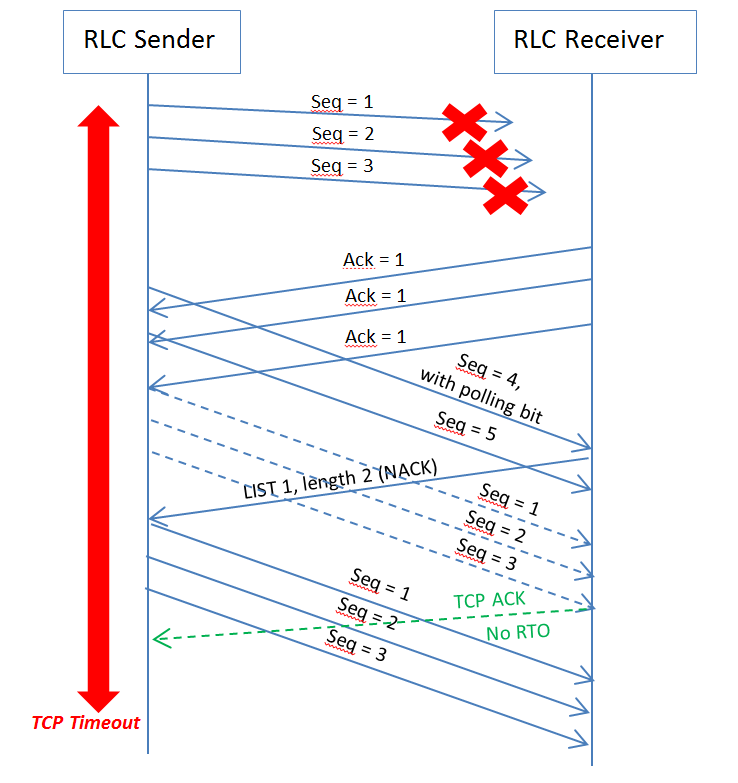
\includegraphics[width=0.45\textwidth]{figs/Win.png}
\caption{Win: RLC Fast Re-Tx avoid a TCP RTO}
\label{fig:win}
\end{figure}

\begin{figure}[h!]
\centering
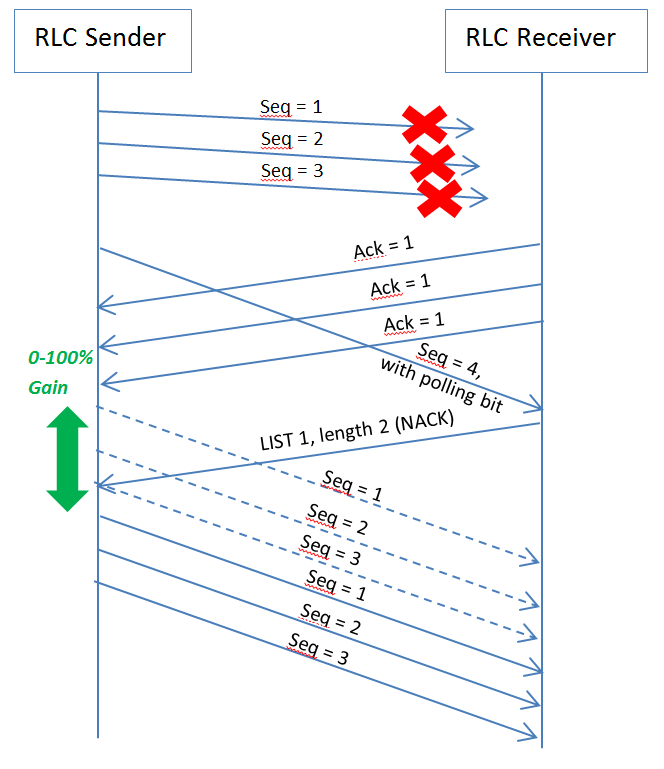
\includegraphics[width=0.45\textwidth]{figs/Draw_plus.png}
\caption{Draw Plus: the predication accuracy is more than 50\%}
\label{fig:draw.plus}
\end{figure}

\begin{figure}[h!]
\centering
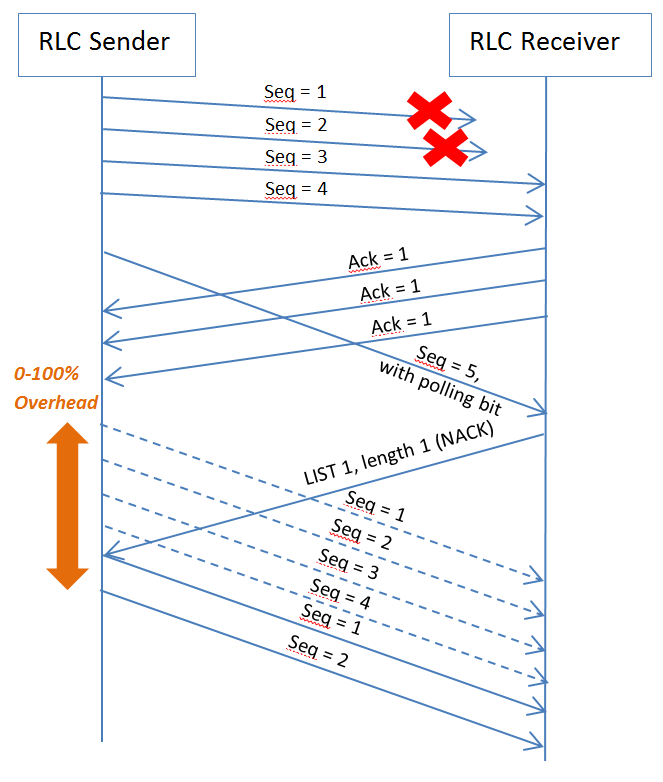
\includegraphics[width=0.45\textwidth]{figs/Draw.png}
\caption{Draw Minus: the predication accuracy is less than 50\%}
\label{fig:draw.minus}
\end{figure}

\begin{figure}[h!]
\centering
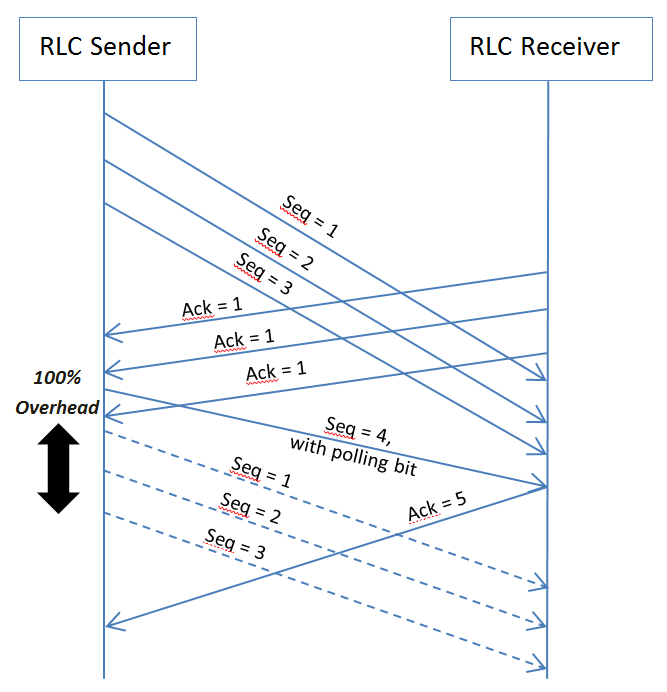
\includegraphics[width=0.45\textwidth]{figs/Loss.png}
\caption{Loss: all predications fail}
\label{fig:loss}
\end{figure}

As we can see from Table~\ref{tab:rlc.fast.sim}, around 75\% of the time we will have benefit on RLC latency reduction if we count the "Win" and "Draw\_{}Plus". The overall RLC delay could be reduced by \textit{2.66\%} over all the RRC state based on trace simulation analysis. If we break down the cost-benefit over different RRC states, the RLC RTT latency could reduce by up to \textit{35.69\%} over initial FACH state or FACH promotion transitions. Therefore, we could have a large latency benefit over the initial period of data transmission.


% Cost-Benefit Table
\begin{table}[h!]
\begin{tabularx}{0.48\textwidth}{ | c | X |}
	\hline
	\textbf{Case Name} & \textbf{Percentage of Occurrence (\%)} \\
	\hline\hline
  	Win & 10.32$\pm$1.89 \\
  	\hline
  	Draw\_{Plus}* & 64.68$\pm$8.32 \\
  	\hline
  	Draw\_{Minus} & 20.63$\pm$3.45 \\
  	\hline
  	Loss & 4.25$\pm$0.06 \\
  	\hline
\end{tabularx}
* The Draw\_{Plus} case excludes the percentage of Win
\caption{The RLC Fast Re-Tx Cost-Benefit Table}
\label{tab:rlc.fast.sim}
\end{table}


\label{sec:eval}

          % 4.0 pg
\section{Future Work}
\label{sec:future}

\subsection{User Study}
We would like to evaluate our real-time user feedback tool with main stream user interactive applications. One of the recent post suggested that the 53\% of the smartphone users listens to Internet radio~\cite{internet.radio}. There are two popular Internet radio applications: TuneIn~\cite{tunein} and Pandora~\cite{pandora}. We will conduct a user study to collect real-time feedback from users when they are listening to Internet radio. Then we could use the cross-layer mapping to identify the root causes for bad QoE periods.

\subsection{Comprehensive Analysis}
We would like to compare the performance across different network carriers and under various of network conditions. Utilizing the cross-layer mapping tool, we will have a better understanding of the implementation difference between carriers, and the trade-off of those design decisions. Previous studies suggested link quality and traffic load could affect cellular network performance~\cite{loadsense,bartendr}. We are also thinking that the actual implementation of lower layer protocol could also be a contributor. That requires to perform a comprehensive analysis on various network carriers and distinguished network conditions.

          % 0.5 pg
\section{Related Work}

Previous work has been done on measuring the power and performance characteristics of 3G RRC state machines~\cite{3g_rrc} as well as 4G LTE networks~\cite{4g_rrc, drx_analysis} in controlled environments, as well as specific features of those networks such as DRX~\cite{drx}.  Work has also been done on exploring the implications on application performance of RRC state and inadequacies in how mobile applications deal with RRC state~\cite{aro}.  

We expand upon this work by implementing an RRC inference method that can be integrated into a measurement tool intended for non-experts. It can automatically infer the RRC state machine of any network type, allowing anomalous or unexpected behavior to be measured, unlike previous work that assumes that devices follow the ideal behavior defined in the specification. We also focus on \emph{transient states} we observe at the RLC level related to promotions and demotions, and their impact on higher-layer performance.   Work by Souders~\cite{souder} measures RRC state machines on client devices, but being a browser-based solution it is not able to account for background activity on the phone or varying network types, measure performance data as accurately as an application can, or observe RLC-level behavior.

Other work has been done on optimizing the use of the cellular network based on 3G or 4G specific phenomena. RadioJockey~\cite{radiojockey} investigates how to effectively trigger fast dormancy based on network traffic patterns, and TailEnder~\cite{tailender} and work by Deng et al.~\cite{trafficaware} propose a method of scheduling data transfers to minimize energy consumption without impacting user-perceived performance.


Related to our RLC fast retransmission proposal, a previous study provides cross comparison analysis over the TCP and RLC protocols, and optimizes the default protocol parameters~\cite{opt.tcp.rlc}. Their primary goal is to improve the performance behavior by introducing TCP congestion control mechanism into the RLC layer. However, their traces are purely generated from simulation software, whereas we use real traffic traces. 

More generally, work has been done to measure performance characteristics of cellular networks and networks on mobile devices. The Livelab project~\cite{livelab} also makes use of users running a measurement app on their phones. A wide range of findings on how users interact with mobile devices have been published, including  measuring web usage in the wild~\cite{livelab-webusage}. Work by Halepovic et al.,~\cite{http_measure} presents a method of passively measuring HTTP transaction latency. Work by Gember et al.,~\cite{incontext} determines how to accurately measure user-perceived performance on user devices. JamLogger~\cite{jamlogger} is an ongoing project to collect general performance and user activity on mobile devices. Our work is complementary to these studies.


%Beyond deployments and testbeds: Experiences with public usage on vehicular WiFi hotspots

%Aditya Akella 	University of Wisconsin
%    Obtaining Representative Measurements of Cellular Network Performance 
%    Explores other factors (network traffic, location etc) that effects measurements
%    Identify that a wide range of factors can affect measurements - we care about relative values
%
%Aruna Balasubramanian 	UW
%     Energy Consumption in Mobile Phones: A Measurement Study and Implications for Network Applications 
%        Tail energy: TailEnder: schedule to avoid tail times

%Joel Sommers 	Colgate University
%    Are Smaller Packets Less Likely to be Lost?:
%    for cellular

% Jamlogger: collects a variety of system statistics periodically in the background; does not have the same challenges as a system looking for specific data, both in measurement cost and in scheduling.  Mobiperf also is not concerned with covering location in the same way and does not have the same challenges.

% LiveLab: Measuring Wireless Networks and Smartphone Users in the Field
% MEasure general real-world smartphone usage and wireless networks. Also uses interrupt-based logging, periodic logging, and collecting when idle.  Hitch-hike onto existing wakeups.  Vary frequency based on context.  More general measurements.  They don't describe power in detail, though - it's a short pape
       % 2.0 pg
\section{Conclusions}
\label{sec:conc}

From the RRC state inference model, I evaluated the latency across each RRC state and state transitions. I observed the extra latency in the FACH state and FACH promotion transitions. Utilizing the QxDM monitoring tool, we have a better visibility over RLC layer traffic information. I wrote a QxDM log parser and analyzer to cross mapping the transport layer and data link layer information, and identified the root cause of abnormal delays cause by channel contention and imperfection in the RLC protocol. I proposed a RLC \textit{Fast Re-Tx} mechanism to actively response to the PDU loss, and evaluated the delay cost-benefit over real-time traces. The latency reduction over FACH and FACH promotion state is up to \textit{35.69\%}, and it could also reduce the overall latency by \textit{2.66\%}. Therefore, the RLC \textit{Fast Re-Tx} mechanism could enhance the user mobile experience by introducing less delays, especially during the initial states of data transmission.
          % 0.25 pg
\section{Acknowledgments}

We would like to thank Yihua Guo, Qi Chen, Sanae Rosen, and Z. Morley Mao for their valuable comments on this report. We would also like to appreciate the support from TMobile.

\label{sec:ack}


           % 0.25 pg

%Uncomment this line if your paper has / uses end notes
%\theendnotes

%\footnotesize
\raggedright
\sloppy
\bibliographystyle{abbrv}
\bibliography{bib}


\end{document}

